\documentclass[17pt]{beamer}

\usepackage[utf8]{vietnam}
\usepackage[vietnamese]{babel}
\usepackage{amsmath}
\usepackage{amsfonts}
\usepackage{amssymb}
\usepackage{graphics}
\usepackage{caption}
\usepackage{booktabs}
\usepackage{hyperref}
\usepackage{graphicx}
\usepackage{tikz}
\usepackage{listings}
\usepackage{xcolor}

\usetheme{Madrid}
\usecolortheme{beaver}

% -------------------------------------------------------
% Thông tin nhóm
% -------------------------------------------------------
\title[BTL XSTK]
{Phân Tích và Dự Đoán Giá Phát Hành GPU}
\subtitle{Dựa Trên Các Thông Số Kỹ Thuật}

\author[Nhóm BTL]
{
  Trần Gia Tường (2313835) \and
  Trần Nhật (2412490) \and
  Trương Minh Triết (2413604) \and
  Vũ Đại Dương (2410638)
}

\institute[HCMUT]{
  GVHD: Huỳnh Thái Duy Phương \\[0.2em]
  Khoa Khoa học \& Kỹ thuật Máy tính \\
  Trường Đại học Bách Khoa -- ĐHQG TP.HCM
}

\date[NH 2025--2026]{TP. Hồ Chí Minh, 2026}

\logo{
\includegraphics[scale=0.35]{hcmut.png}}

% -------------------------------------------------------
% Màu sắc cho code listing
% -------------------------------------------------------
\definecolor{dkgreen}{rgb}{0,0.6,0}
\definecolor{codegray}{rgb}{0.5,0.5,0.5}
\lstset{
  language=R,
  basicstyle=\ttfamily\tiny,
  keywordstyle=\color{blue},
  commentstyle=\color{dkgreen},
  stringstyle=\color{red},
  breaklines=true,
  showstringspaces=false,
  frame=single,
}

% -------------------------------------------------------
\begin{document}

% ---- Trang bìa ----
\frame{\titlepage}

% ---- Mục lục ----
\begin{frame}{Nội dung trình bày}
  \tableofcontents
\end{frame}

% ================================================================
\section{Đối tượng, Mục tiêu và Kết quả Hướng tới}
% ================================================================

\begin{frame}{Bộ dữ liệu}
  \begin{itemize}
    \item Bộ dữ liệu \textbf{All\_GPUs.csv} từ Kaggle (tác giả: Iliasse Kkaf)
    \item Hơn \textbf{3.400 GPU} từ NVIDIA, AMD và Intel
    \item \textbf{34 thuộc tính}; nhóm chọn \textbf{8 biến} chính:
  \end{itemize}
  \begin{columns}
    \column{0.5\textwidth}
      \begin{itemize}
        \item \texttt{core\_speed}
        \item \texttt{tdp}
        \item \texttt{memory\_size}
        \item \texttt{memory\_type}
      \end{itemize}
    \column{0.5\textwidth}
      \begin{itemize}
        \item \texttt{memory\_bus}
        \item \texttt{manufacturer}
        \item \texttt{release\_year}
        \item \textbf{\texttt{release\_price}} (biến mục tiêu)
      \end{itemize}
  \end{columns}
\end{frame}

\begin{frame}{Bối cảnh và Mục tiêu}
  \begin{block}{Câu hỏi nghiên cứu}
    Thông số kỹ thuật nào thực sự \alert{quyết định giá} GPU?
    NVIDIA có đắt hơn AMD đáng kể không?
  \end{block}
  \vspace{0.5em}
  \textbf{Mục tiêu cụ thể:}
  \begin{enumerate}
    \item Phân tích thống kê mô tả và phân phối giá GPU
    \item Kiểm định giả thuyết về sự khác biệt giá giữa NVIDIA -- AMD
    \item Xây dựng mô hình hồi quy dự đoán \texttt{release\_price}
  \end{enumerate}
\end{frame}

% ================================================================
\section{Cơ sở Lý thuyết}
% ================================================================

\begin{frame}{Các phương pháp thống kê sử dụng}
  \begin{columns}
    \column{0.5\textwidth}
      \textbf{Thống kê mô tả}
      \begin{itemize}
        \item Trung bình, trung vị, độ lệch chuẩn
        \item Phát hiện outlier (IQR)
        \item Phân phối và biểu đồ
      \end{itemize}
    \column{0.5\textwidth}
      \textbf{Kiểm định \& Mô hình}
      \begin{itemize}
        \item Kiểm định t (so sánh 2 nhóm)
        \item Kiểm định Wilcoxon
        \item Hồi quy tuyến tính bội
        \item Đánh giá: $R^2$, RMSE, MAE
      \end{itemize}
  \end{columns}
\end{frame}

% ================================================================
\section{Xử lý Dữ liệu}
% ================================================================

\begin{frame}{Quy trình xử lý dữ liệu}
  \begin{figure}
    \centering
    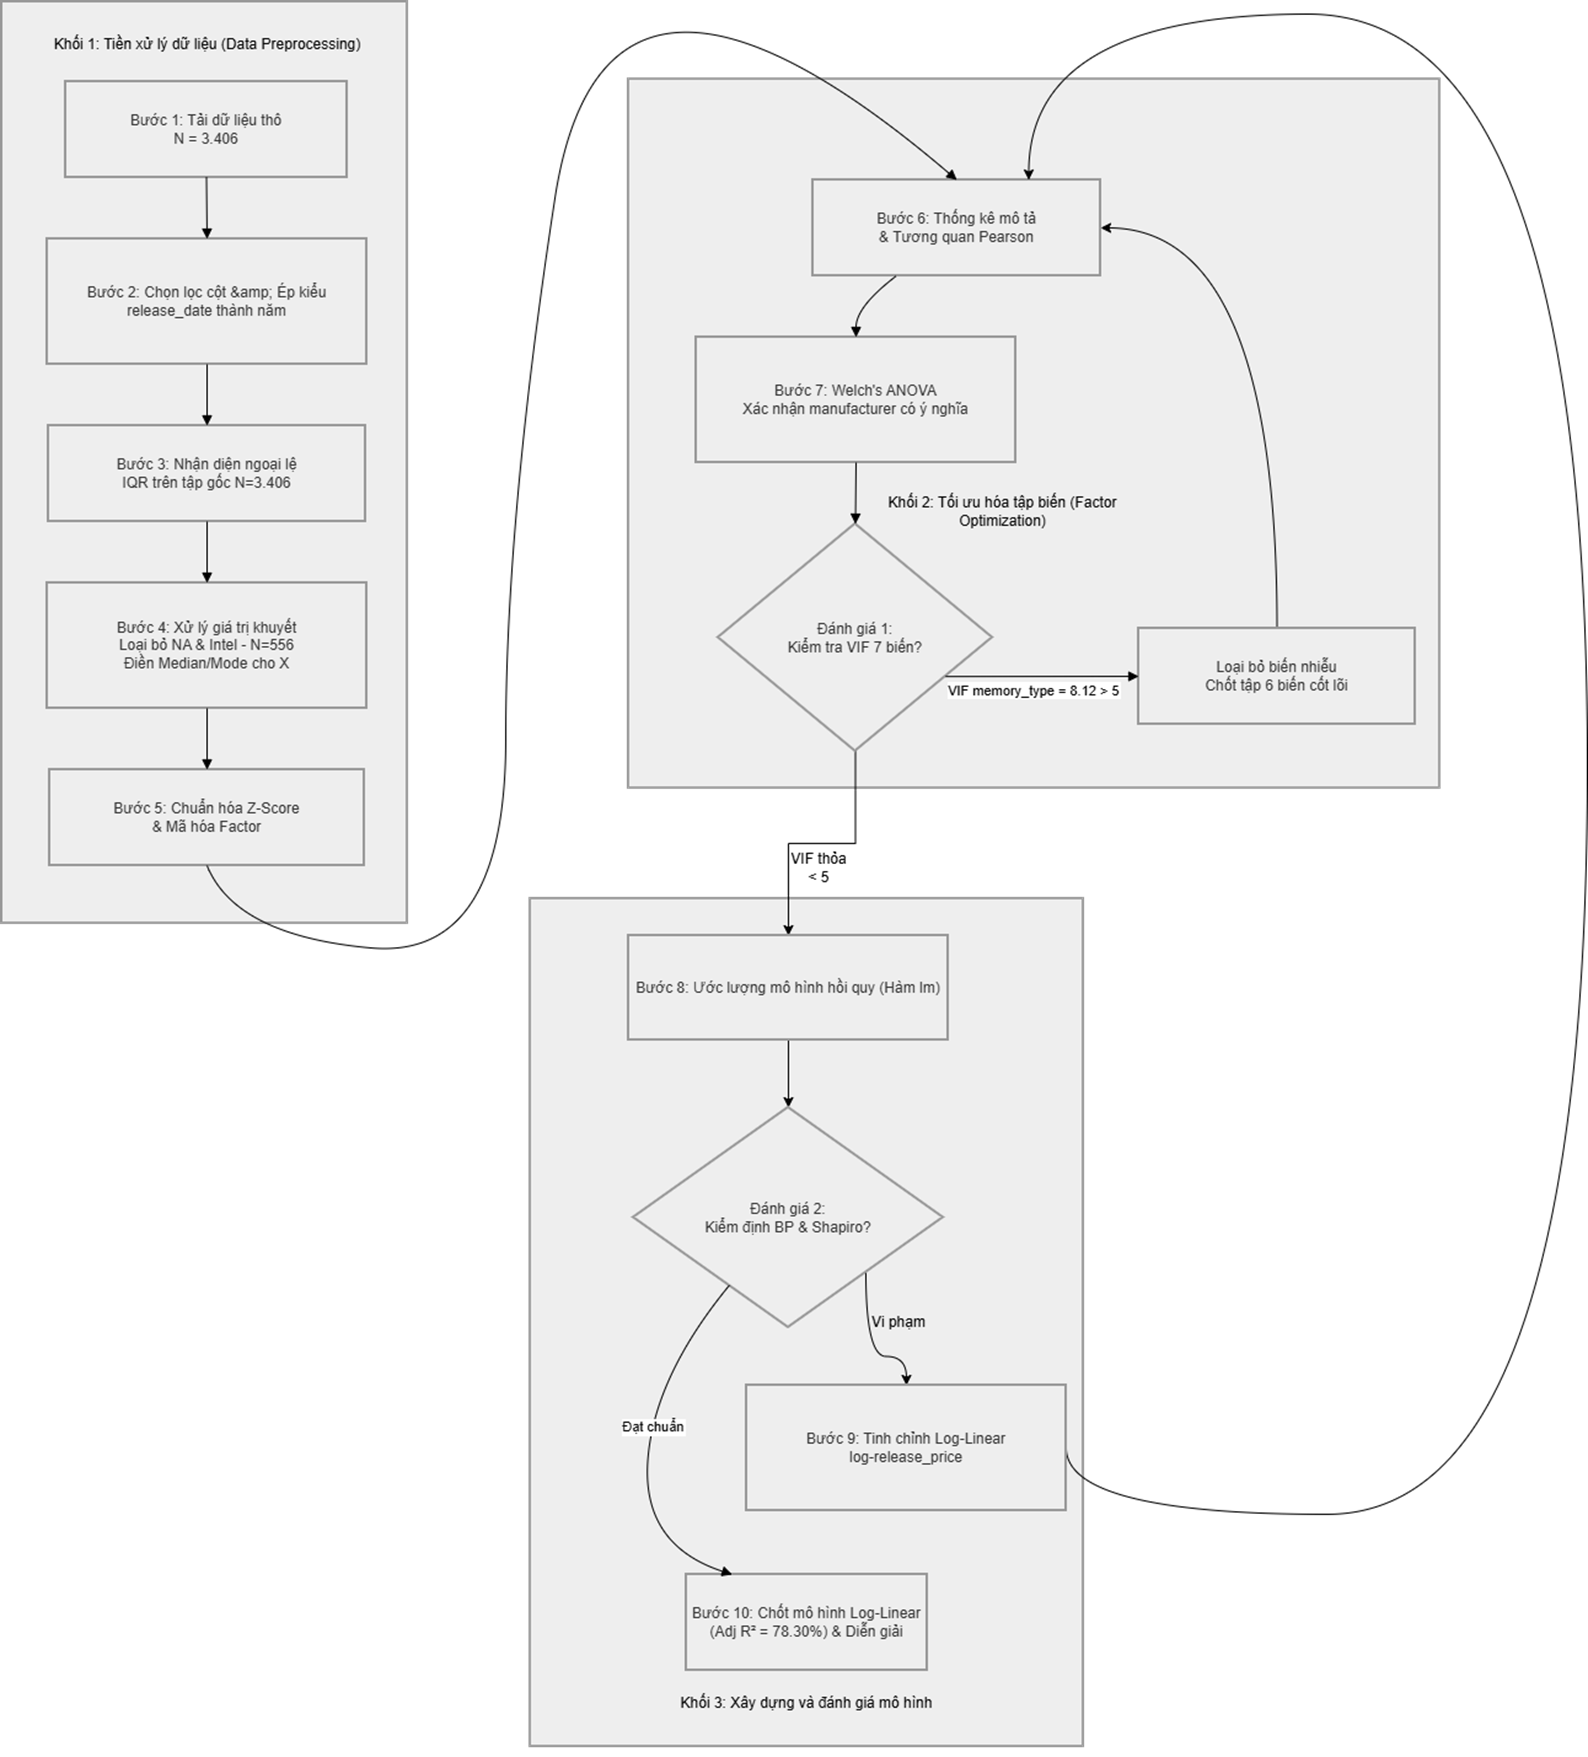
\includegraphics[width=0.85\textwidth]{figures/chart_quy_trinh_xu_ly.png}
    \caption{Quy trình làm sạch và chuẩn hóa dữ liệu}
  \end{figure}
\end{frame}

\begin{frame}{Phát hiện và xử lý Outlier}
  \begin{figure}
    \centering
    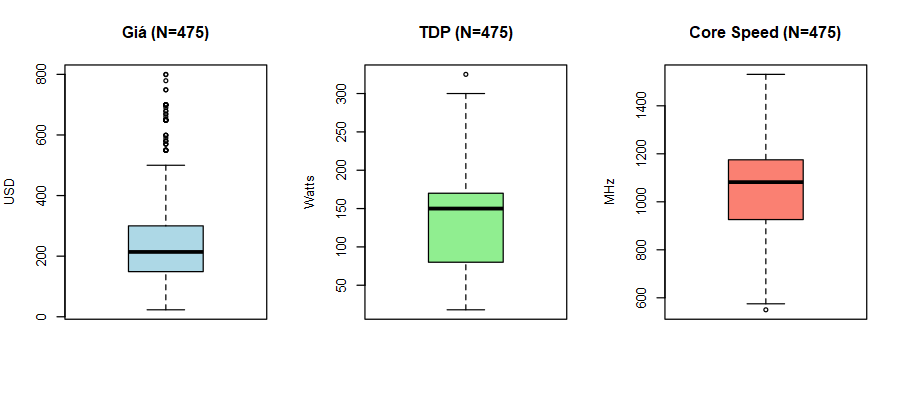
\includegraphics[width=0.85\textwidth]{figures/boxplot_outliers.png}
    \caption{Boxplot phát hiện outlier theo nhà sản xuất}
  \end{figure}
\end{frame}

% ================================================================
\section{Kết quả Thu được}
% ================================================================

\begin{frame}{Kết quả mô hình hồi quy}
  \begin{figure}
    \centering
    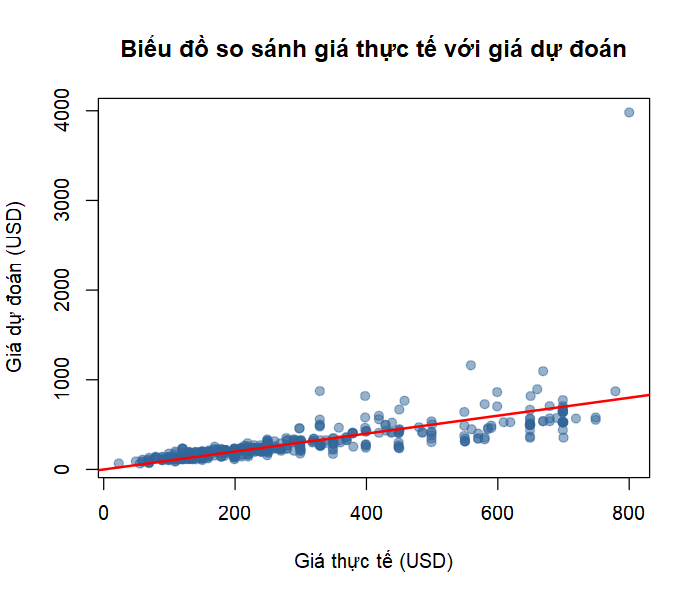
\includegraphics[width=0.78\textwidth]{figures/scatter_actual_vs_predicted.png}
    \caption{Giá thực tế vs. Giá dự đoán (Hồi quy tuyến tính)}
  \end{figure}
\end{frame}

\begin{frame}{Đánh giá mô hình}
  % TODO: điền số liệu từ kết quả R
  \begin{table}
    \centering
    \begin{tabular}{lc}
      \toprule
      \textbf{Chỉ số} & \textbf{Giá trị} \\
      \midrule
      $R^2$           & \ldots \\
      RMSE            & \ldots \\
      MAE             & \ldots \\
      \bottomrule
    \end{tabular}
    \caption{Chỉ số đánh giá mô hình trên tập kiểm tra}
  \end{table}
  \begin{block}{Nhận xét}
    % TODO: thêm nhận xét sau khi có số liệu
  \end{block}
\end{frame}

\begin{frame}{Kiểm định NVIDIA vs. AMD}
  % TODO: điền kết quả kiểm định t/Wilcoxon
  \begin{itemize}
    \item Hypotheses: $H_0$: không có sự khác biệt giá trung bình
    \item Phương pháp: \ldots
    \item p-value: \ldots
    \item Kết luận: \ldots
  \end{itemize}
\end{frame}

% ================================================================
\section{Kết luận và Đề nghị}
% ================================================================

\begin{frame}{Kết luận}
  \begin{block}{Những gì đã làm được}
    \begin{itemize}
      \item Phân tích thống kê toàn diện bộ dữ liệu GPU
      \item Xây dựng và đánh giá mô hình hồi quy dự đoán giá
      \item Kiểm định sự khác biệt giá giữa NVIDIA và AMD
    \end{itemize}
  \end{block}
  \begin{block}{Hạn chế và hướng phát triển}
    \begin{itemize}
      \item Dữ liệu thiếu một số năm gần đây (GPU AI thế hệ mới)
      \item Có thể thử mô hình phi tuyến (Random Forest, XGBoost)
    \end{itemize}
  \end{block}
\end{frame}

\begin{frame}[plain]
  \begin{center}
    {\Huge \textbf{Cảm ơn thầy và các bạn}}\\[1em]
    {\large đã lắng nghe!}\\[2em]
    \textit{Nhóm xin nhận câu hỏi.}
  \end{center}
\end{frame}

\end{document}
